% Drawing 69/04-1 -- folder 69, batch 04, archive page 62 (PDF page 63).
% Transcription: trois petits graphes en zigzag (lettres « M » et « W » faites de sommets et d'arêtes), deux d'entre eux entourés de boucles, une ligne brisée en créneau, un chevron.
% Kind: zigzag graphs (M, W), loops, a crenel line, a chevron. Method 2 (schematic redraw from the facsimile). Status: ok.
% Notes: Half-sheet of Institut de Mathematiques letterhead (printed heading not drawn). Top centre: an M-shaped graph on three vertical strokes (the left one broken under its upper dot), heavy dots at the top and middle of the left stroke, at the middle and bottom of the middle one and at the middle of the right one; two rising diagonals (left bottom to middle top, middle bottom to right top); a short stroke falling from the top left dot, a second short stroke beside the middle dot, a short stroke at the foot of the right one; two thin strokes: a curve left of the middle stroke, from its middle dot down to its foot, and a line from the middle dot towards the top of the right one. Right of it: a chevron with a small angle before it, and below them a crenel line. Top right: a W of six vertices (thick) inside three long open loops running off the right edge of the crop (a short separate stroke at the lower right of the first). Bottom left: two crossing loops (an outer one from a hook at its top round the left to a heavy end at the lower right, an inner one closing on it at the left) and a third, lower open loop, with three vertical strokes (the last thick); bottom middle: a loop with four dots and, under it, an M of thick strokes (a crossed N) with an I beside it, above a second loop. Vertices placed once, the zigzags drawn as single polylines through them. Not drawn: the two long diagonal strokes across the sheet, the computations, and the small letters written in and beside the bottom loops (xi', eta, eta' and the like). Second pass 2026-11-14 (issue 147, Claude Opus 5.5): the seven loops, drawn before as ellipses, redrawn as his open freehand curves from high-contrast grid overlays at 30 to 60 px per unit; the two thin strokes of the top M, too faint at the first pass, read on a high-contrast overlay at 45 px per unit and drawn; the four dots of the bottom middle moved by up to 0.5 unit. The rasterised redraw laid over the crop: every stroke on its ink to within about half a unit. Not compiled (no TeX engine in the session).
% Coordinates: 1 unit = 1 mm = 1/100 of the crop width (bbox in page fractions: [0.05, 0.12, 0.95, 0.5]).
% Redrawn by Claude (claude-opus-5-5), issue #73, 2026-11-09; not checked by a human; not compiled (no TeX in the session).
% Checked by Claude (claude-opus-5-5) 2026-11-14 (issue #147, second pass): strokes redrawn from the 300 dpi colour render of the 250 ppi scan, coordinates read on a grid overlay and checked by overlaying the rasterised redraw; not compiled (no TeX in the session). Not checked by a human. Status: ok.
% Rights: reproduces part of the work -- behind RENDER_TRANSCRIPTS, never published by itself.
\documentclass[tikz,border=3pt]{standalone}
\usepackage{amsmath,amssymb}
\usetikzlibrary{patterns,arrows.meta}
\tikzset{pencil/.style={black!45}, struck/.style={black!35}, mark/.style={circle,draw,inner sep=1.3pt}, pt/.style={circle,fill,inner sep=0.9pt}, opt/.style={circle,draw,fill=white,inner sep=1.1pt}}
\begin{document}
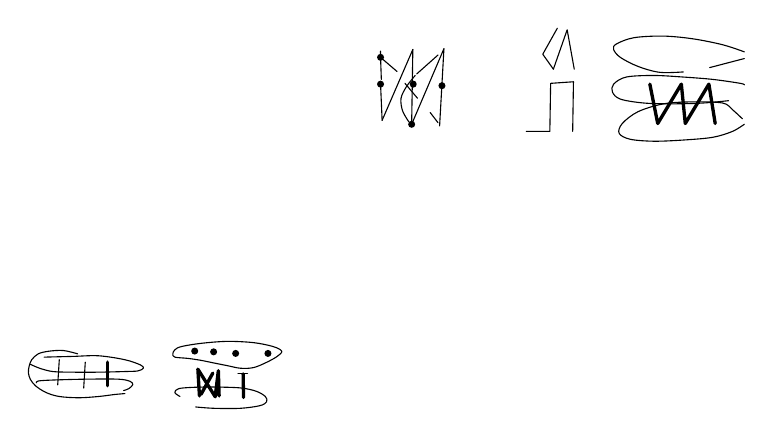
\begin{tikzpicture}[x=1mm,y=1mm,line cap=round,line join=round,font=\scriptsize]
\draw (53.8,-13.3) -- (53.8,-14.1) -- (53.9,-16.9);
\draw (53.8,-17.5) -- (54,-22.1);
\draw (57.9,-13.1) -- (57.75,-22.6);
\draw (61.85,-13) -- (61.3,-22.8);
\draw (54,-22.1) -- (57.9,-13.1);
\draw (57.75,-22.6) -- (61.85,-13);
\draw (53.8,-14.1) -- (55.9,-15.9);
\draw (56.9,-17.4) -- (58.5,-19.3);
\draw (60.1,-21.1) -- (61.1,-22.4);
\draw plot[smooth, tension=0.55] coordinates {(58.2,-16.4) (57.1,-17.8) (56.4,-19.3) (56.6,-20.9) (57.4,-22.3)};
\draw (58.4,-16.2) -- (61.1,-13.8);
\node[pt] at (53.8,-14.1) {};
\node[pt] at (53.8,-17.5) {};
\node[pt] at (57.95,-17.5) {};
\node[pt] at (57.75,-22.6) {};
\node[pt] at (61.6,-17.7) {};
\draw (76.25,-10.4) -- (74.4,-13.7) -- (75.75,-15.6);
\draw (75.75,-15.6) -- (77.5,-10.6) -- (78.4,-15.6);
\draw (72.3,-23.5) -- (75.3,-23.5) -- (75.4,-17.4) -- (78.3,-17.2) -- (78.2,-23.5);
\draw[very thick] (88,-17.5) -- (89,-22.5) -- (92,-17.5) -- (92.5,-22.5) -- (95.5,-17.5) -- (96.3,-22.5);
\draw plot[smooth, tension=0.55] coordinates {(92.25,-15.95) (89.25,-16) (86.5,-15.25) (84.25,-14.1) (83.4,-13.1) (83.75,-12.4) (86,-11.6) (89.75,-11.4) (93.5,-11.75) (97.25,-12.5) (100,-13.4)};
\draw (95.6,-15.4) -- (100,-14.25);
\draw plot[smooth, tension=0.55] coordinates {(100,-17.6) (99.5,-17.4) (96,-16.9) (92.25,-16.6) (88.5,-16.4) (85,-16.6) (83.4,-17.5) (83.25,-18.5) (84.25,-19.4) (87.25,-19.9) (91,-20) (94.75,-19.9) (98,-19.6)};
\draw plot[smooth, tension=0.55] coordinates {(99.75,-21.9) (98.5,-20.75) (97.25,-19.9) (93.5,-19.75) (89.75,-20) (86.5,-21) (84.5,-22.5) (84.1,-23.75) (85.5,-24.5) (88.5,-24.75) (92.25,-24.6) (96,-24.25) (98.5,-23.5) (100,-22.6)};
\draw plot[smooth, tension=0.55] coordinates {(15.33,-51.75) (13.5,-51.33) (11.67,-51.42) (10.33,-51.75) (9.5,-52.5) (9.17,-53.33) (9.08,-54.17) (9.33,-55) (10,-55.83) (11.33,-56.67) (13,-57.17) (15.5,-57.33) (18,-57.17) (20,-56.92) (21.33,-56.8)};
\draw plot[smooth, tension=0.55] coordinates {(11.08,-52.17) (14.67,-52.08) (18,-52) (21.33,-52.5) (23.33,-53.17) (23.67,-53.58) (23,-53.92) (21.33,-54) (18,-54.08) (14.67,-54.08) (12.17,-54) (10.5,-53.58) (9.33,-53.08)};
\draw plot[smooth, tension=0.55] coordinates {(10.08,-55.42) (10.33,-55.2) (12.17,-55.08) (16.33,-54.97) (20.5,-54.97) (22,-55.25) (22.33,-55.67) (21.83,-56.17) (21.17,-56.42)};
\draw (13,-52.5) -- (12.8,-55.7);
\draw (16.3,-52.8) -- (16.1,-56.1);
\draw[very thick] (19.1,-52.8) -- (19.1,-55.8);
\draw plot[smooth cycle, tension=0.55] coordinates {(27.67,-51.25) (28.5,-50.83) (31,-50.42) (34.33,-50.17) (37.67,-50.33) (40.17,-50.83) (41.25,-51.42) (40.67,-52.08) (39.33,-52.83) (37.67,-53.5) (36,-53.58) (34.33,-53.25) (32.67,-52.92) (31,-52.58) (29.33,-52.33) (27.67,-52.17) (27.42,-51.75)};
\draw plot[smooth, tension=0.55] coordinates {(28.33,-57.17) (27.67,-56.67) (28.17,-56.17) (30.17,-56) (32.67,-55.97) (36,-56.08) (38,-56.5) (39.17,-57.17) (39.33,-57.83) (38.5,-58.33) (36,-58.67) (32.67,-58.67) (30.33,-58.5)};
\draw[very thick] (30.8,-57.1) -- (30.6,-53.7) -- (32.8,-57.2) -- (33.2,-53.9) -- (33.3,-57.1);
\draw[very thick] (31,-56.9) -- (32.5,-54.2);
\draw[very thick] (36.35,-54.3) -- (36.4,-57.3);
\draw (35.7,-54.3) -- (36.9,-54.3);
\node[pt] at (30.2,-51.4) {};
\node[pt] at (32.6,-51.5) {};
\node[pt] at (35.4,-51.7) {};
\node[pt] at (39.5,-51.7) {};
\end{tikzpicture}
\end{document}
